\documentclass[11pt,a4paper]{article}
\usepackage[margin=2.4cm]{geometry}
\usepackage{graphicx}
\usepackage{amsmath}
\usepackage{booktabs}
\usepackage[colorlinks=true,linkcolor=black,urlcolor=blue,citecolor=black]{hyperref}
\usepackage{caption}
\captionsetup{font=small,labelfont=bf}
\graphicspath{{../Plot/}}
\setlength{\parskip}{0.4em}
\setlength{\parindent}{0pt}

\title{\bfseries A Rederivation of the AYO ExoEarth Yield Formalism,\\
and HWO Yields for a Mass-Selected Planet Sample\\[0.3em]
\large in a Narrowed Habitable Zone}
\author{Prepared in the \texttt{yields} vaibify project}
\date{\today}

\begin{document}
\maketitle

\begin{abstract}
\noindent
This report rederives the Altruistic Yield Optimization (AYO) exoEarth-candidate yield
formalism of Stark et al.\ (2014, 2019, 2024) from the published equations and parameter
tables, and uses it to answer a counterfactual: what would the Habitable Worlds Observatory
(HWO) baseline yield if the planet sample were defined by mass, $0.5$--$2\,M_\oplus$ with
$R = M^{0.27}$, and if the habitable zone were $0.96$--$1.20$~AU for the Sun rather than the
conservative $0.95$--$1.67$~AU, scaled by $\sqrt{L_\star}$ for every star. Integrating the
SAG13 occurrence law over the redefined box gives
$\eta = @@ETARMED@@^{+@@ETARUP@@}_{-@@ETARDN@@}$ against
$@@ETACMED@@^{+@@ETACUP@@}_{-@@ETACDN@@}$ for the canonical box, a ratio of
$@@OCCRATIO@@^{+@@OCCRATIOUP@@}_{-@@OCCRATIODN@@}$ that is independent of the overall
normalisation. The full survey optimization gives a \emph{yield} ratio of
$@@YRATIO@@^{+@@YRATIOUP@@}_{-@@YRATIODN@@}$, materially larger than the occurrence ratio,
because a smaller expected detection count frees characterization time and because truncating
the outer habitable zone preferentially removes the faintest, most expensive planets. The
baseline 6\,m design yields a median of @@REDEFMED@@ exoEarth candidates under the redefined
selection, against @@CANONMED@@ canonically, and the probability of reaching the 25-planet
goal falls from @@CANONP25@@\% to @@REDEFP25@@\%.
\end{abstract}

\tableofcontents

\section{The question, and what it required}

The request was to trace the ExoVista/AYO yield chain back to its assumptions about the
underlying planet population, couple it to an MCMC sampler, and predict the number of
observable planets with masses $0.5$--$2\,M_\oplus$ and radii $R = M^{0.27}$ around FGK stars,
under a habitable zone narrowed to $0.96$--$1.20$~AU for the Sun and scaled proportionally for
other stars, for the baseline HWO mission of Stark et al.\ (2024).

Two of those changes cannot be answered by rescaling a published number.

Changing the planet box changes \emph{which integral} of the occurrence-rate density is
reported, which is a pure population-model question and is answered in
Section~\ref{sec:occurrence}. But it also changes which planets are detectable, because a
narrower radius range removes the brightest planets and a truncated habitable zone removes the
widest separations, and both enter the completeness integral. Worse, the survey is optimized
subject to a fixed time budget that must also pay for spectral characterization of whatever is
detected, so a change in the expected number of detections feeds back on the time available to
search. Stark et al.\ (2024, \S3.5) make this explicit when they call $\eta_\oplus$ an
\emph{actionable} source of uncertainty. The consequence is that yield is not proportional to
$\eta$, and the question can only be answered by re-running the optimization.

\section{What is, and is not, reproducible from the published record}

The AYO \emph{code} is not available: the Data and Code Availability statement of Stark et al.\
(2024) notes that NASA regulations govern its release and directs readers to contact the
corresponding author. The AYO \emph{formalism}, however, is published in full. Stark et al.\
(2019) reproduce the exposure-time equations explicitly, and Stark et al.\ (2024) Tables 1 and
2 give every astrophysical and mission parameter the baseline design uses.

\begin{table}[htbp]
\centering
\small
\begin{tabular}{p{5.6cm}p{4.2cm}p{5.2cm}}
\toprule
\textbf{Ingredient} & \textbf{Status} & \textbf{What this project did} \\
\midrule
Exposure-time and count-rate equations & Published (Stark+2019) & Implemented verbatim \\
Mission, detector, throughput parameters & Published (Stark+2024 Tab.~2) & Transcribed \\
EEC box, albedo, exozodi model & Published (Stark+2024 Tab.~1) & Transcribed \\
Equal-slope optimization principle & Published (Stark+2014) & Implemented \\
Target catalog (HPIC) & Not distributed here & Rebuilt from Gaia DR3 + Hipparcos \\
$\Upsilon_c(x,y)$, $I(x,y)$ coronagraph maps & \textbf{Not published} & Parametrized, then calibrated \\
Per-star completeness / time allocation & Not published & Recomputed \\
\bottomrule
\end{tabular}
\caption{The published record supports a rederivation everywhere except the simulated
coronagraph maps, which are the output of detailed diffraction modelling that the papers
describe but do not distribute.}
\end{table}

The single genuine gap is the pair of simulated coronagraph maps. Section~\ref{sec:calibration}
explains how it is handled and, more importantly, how the report reports its own exposure to it.

\section{Method}

\subsection{Population model}
\label{sec:occurrence}

Planets are drawn from the SAG13 broken power law, in the small-planet regime relevant here,
\begin{equation}
\frac{\mathrm{d}^2 N}{\mathrm{d}\ln R\,\mathrm{d}\ln P} = \Gamma\, R^{\alpha} P^{\beta},
\qquad \Gamma = 0.38,\ \alpha = -0.19,\ \beta = 0.26,
\end{equation}
with $R$ in Earth radii and $P$ in years. Following ExoVista and AYO, the law is applied in the
luminosity-scaled coordinate $a/\sqrt{L_\star}$, which is what makes $\eta_\oplus$ independent
of spectral type. Integrated over the canonical HabEx/LUVOIR exoEarth-candidate box --- the
conservative habitable zone $0.95$--$1.67$~AU with $0.8\,(a/\mathrm{EEID})^{-0.5} < R < 1.4$ ---
this returns $\eta_\oplus = 0.240$, reproducing the value Stark et al.\ adopt. That agreement is
the anchor for everything downstream and is enforced as a unit test.

The redefined box replaces the radius limits with a mass selection, $0.5 < M/M_\oplus < 2$ with
$R = M^{0.27}$, giving $0.829 < R/R_\oplus < 1.206$, and narrows the habitable zone to
$0.96$--$1.20$ scaled AU. The exponent $0.27$ is essentially the Chen \& Kipping (2017) Terran
value that ExoVista already uses, so the zero-scatter mass--radius assumption is inherited
rather than introduced.

\subsection{Radiometry and exposure time}

Exposure times follow Stark et al.\ (2019):
\begin{equation}
\tau = \left(\mathrm{S/N}\right)^2 \frac{\mathrm{CR_p} + 2\,\mathrm{CR_b}}{\mathrm{CR_p}^2},
\qquad
\mathrm{CR_p} = F_0\,10^{-0.4(m_\lambda + \Delta\mathrm{mag_p})}\,A\,\Upsilon_c\,T\,\Delta\lambda ,
\end{equation}
with backgrounds from leaked starlight, local zodiacal light, exozodiacal light and the
detector. Stellar fluxes are computed from a blackbody at the catalogued $T_{\rm eff}$ and
radius rather than from apparent magnitudes, which removes any dependence on a bandpass zero
point or colour transformation; this is verified against the Sun's absolute $V$ magnitude to
better than 5\%. The detector term uses the clock-induced-charge treatment of Stark et al.\
(2019) Eq.~9, whose coefficient $6.73 = -[1 + W_{-1}(-q/e)]^{-1}$ at $q = 0.99$ is reproduced
independently from the Lambert $W$ function as a test. Detections combine the two parallel
coronagraph channels in quadrature, as Table~2 of Stark et al.\ (2024) specifies.

\subsection{Completeness}

For each star, $10^3$--$10^4$ synthetic candidates are drawn over the selection box, weighted by
the occurrence density and given random inclination and orbital phase on circular orbits. Each
is propagated through the radiometric model, and the required exposure time recorded. A planet
is excluded outright if it falls below the post-processing noise floor
($\Delta\mathrm{mag} > 26.5$), outside the dark zone, or needs more than the two-month exposure
cap. Completeness $C(\tau)$ is then the fraction of \emph{all} injected planets detectable
within $\tau$, so the geometric, photometric and noise-floor losses are already inside it.

\subsection{Equal-slope optimization with characterization}

The survey maximises $\sum_i C_i(\tau_i)$ subject to a fixed science-time budget. The optimum
satisfies the equal-slope condition $\mathrm{d}C_i/\mathrm{d}T_i = \lambda$ for every observed
star, and $\lambda$ is swept until the budget closes; stars whose marginal return never reaches
$\lambda$ drop out of the survey. Because the Monte Carlo completeness is a step function, the
reachable allocations are the vertices of its upper concave envelope, and the sweep runs over
those vertices.

Characterization is charged into the same budget. Each star's cost carries an additional term
\begin{equation}
\eta\,C_i(\tau_i)\left(\tau'\,\tau_{{\rm char},i} + \tau_{\rm overhead}\right),
\end{equation}
so a star expected to deliver more detections also consumes more of the mission. This is the coupling that
makes yield sub-linear in $\eta$, and it is verified by a pair of unit tests: with the
characterization term removed the yield is exactly proportional to $\eta$, and with it present
the proportionality breaks.

\subsection{Occurrence posterior}

The posterior over $(\ln\Gamma, \alpha, \beta)$ is sampled with \texttt{emcee}
(@@POSTSAMPLES@@ samples after burn-in, mean acceptance fraction @@POSTACCEPT@@). The model is
deliberately modest about what it infers. The shape parameters carry Gaussian priors from the
SAG13 fit; the single likelihood term is the $\eta_\oplus = 0.26^{+0.29}_{-0.14}$ (86\%) that
Stark et al.\ (2024) obtain by integrating the Bryson et al.\ (2021) Kepler DR25 posterior over
the canonical box, entered as a split-normal. The posterior is therefore prior-dominated in
$\alpha$ and $\beta$ and likelihood-dominated in the normalisation. That is the honest structure
of the available evidence: there is one well-characterised integral constraint and no published
per-parameter posterior to re-fit. What the sampler buys is not a tighter $\eta$ but a
principled propagation of the same rate law onto a \emph{different} integration domain.

\section{Validation, and how to check it yourself}
\label{sec:calibration}

\subsection{The target catalog}

HPIC is not reachable from this environment, so the target list is rebuilt from Gaia DR3 --- one
of HPIC's two parent catalogs --- yielding @@CATGAIA@@ dwarfs within 50~pc, of which @@CATFGK@@
are FGK. Gaia publishes no astrophysical parameters brighter than $G \approx 3$, which silently
removes $\alpha$~Cen~A and~B, Procyon, $\tau$~Ceti and $\epsilon$~Eridani: precisely the targets
whose habitable zones subtend the largest angles. A Hipparcos supplement restores
@@CATHIP@@ bright stars, with $T_{\rm eff}$ from $B\!-\!V$ and luminosities from absolute
magnitudes plus a Torres (2010) bolometric correction, for @@CATROWS@@ stars in total. Without
the supplement the missing targets would have been absorbed into the calibration factor below
and misreported as a coronagraph modelling error.

\subsection{The calibration gate, and what it does not license}

The parametrized coronagraph stands in for simulated maps, so a single scalar throughput factor
absorbs the residual mismatch, fitted by bisection against the 22.5 exoEarth candidates that
Stark et al.\ (2024) report for the baseline 6\,m design (Figure~\ref{fig:calibration}). The
fitted factor is @@CALFACTOR@@ --- the model needs roughly @@CALFACTORINV@@ times \emph{less}
throughput than the parametrization assumes.

\textbf{The calibrated yield is not evidence of anything.} It is tuned to 22.5 by construction
and will always agree. Only two things about the calibration carry information: that the
\emph{uncalibrated} prediction was already @@CALUNCAL@@ against a published 22.5, and that the
factor needed is within a factor of two of unity. The curve in Figure~\ref{fig:calibration} is
also shallow --- a 42\% cut in throughput costs under 10\% of the yield --- because the survey is
partly limited by the inner working angle and the noise floor rather than by photons. A weak
lever cannot manufacture agreement that was not already close.

\begin{figure}[htbp]
\centering
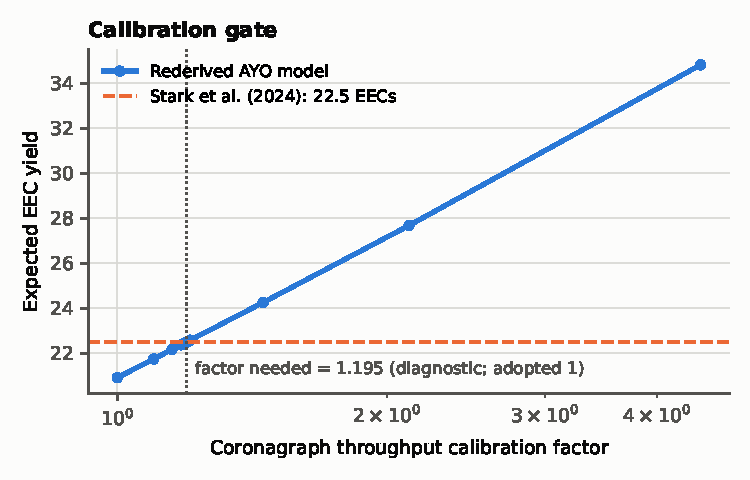
\includegraphics[width=0.62\textwidth]{figCalibration.pdf}
\caption{Modelled yield against the coronagraph throughput calibration factor. The published
22.5-candidate value is met at a factor of @@CALFACTOR@@, and the curve is shallow: a 42\%
reduction in throughput costs under 10\% of the yield.}
\label{fig:calibration}
\end{figure}

\subsection{Checks already passed}

\begin{table}[htbp]
\centering
\small
\begin{tabular}{p{6.2cm}rrp{3.9cm}}
\toprule
\textbf{Quantity} & \textbf{Published} & \textbf{Here} & \textbf{Status} \\
\midrule
$\eta_\oplus$, SAG13 over the canonical box & 0.24 & @@ETASAG13@@ & Independent \\
Expected yield, 6\,m, \emph{before} calibration & 22.5 & @@CALUNCAL@@ & Independent \\
$P_{25}$ including $\sigma_{\eta_\oplus}$, 6\,m & 32\% & @@CANONP25@@\% & Independent \\
Expected yield, 6\,m, after calibration & 22.5 & @@CALYIELD@@ & \textbf{Tuned (not evidence)} \\
\bottomrule
\end{tabular}
\caption{Comparisons against values stated in the text of Stark et al.\ (2024). The first three
were not fitted to; the fourth is the calibration target and is listed only so it is not
mistaken for a result.}
\end{table}

The $\eta_\oplus$ row involves no telescope model at all and tests the population layer alone.
The $P_{25}$ row is the most informative of the three, because it depends on the completeness
model, the optimizer, the characterization budget and the occurrence posterior simultaneously,
and nothing in the pipeline was fitted to it.

\subsection{Checking this yourself, in one command}

\begin{verbatim}
cd explorations && python3 checkAgainstPublishedValues.py --repo-root ..
\end{verbatim}

This reads the step outputs, compares each against the published anchor, prints a pass/fail
table, and writes \texttt{publishedValueComparison.json}. It checks only values stated in the
paper \emph{text}, never values read off a figure, and it tags the calibration row as tuned so
it is never counted as agreement. It also lists the stronger checks below that have not been
run.

\subsection{Stronger checks this report has not run}

Three scalars at a single design point is weak evidence. A scalar can be hit by luck or by
compensating errors; a \emph{curve} cannot. Ranked by how much they would tell you:

\begin{enumerate}
\item \textbf{$P_{25}$ against aperture --- Stark et al.\ (2024) Fig.~15.} The strongest check
available. Four diameters (6, 7, 8, 9\,m), two curves, and a distinctive crossing near 7.1\,m
where the no-$\sigma_{\eta_\oplus}$ curve overtakes the other. Reading off that figure, the
including-$\sigma_{\eta_\oplus}$ curve runs $\approx$ 32.3 / 53 / 67 / 78\%, and the excluding
curve $\approx$ 5.6 / 49 / 89 / 99.5\%. Because the calibration is fitted at 6\,m only, the
7, 8 and 9\,m points are genuine out-of-sample predictions, and reproducing the crossing tests
the \emph{shape} of the aperture scaling rather than any single value. Run A04, A05 and A07 at
\texttt{-{}-diameter-m 7, 8, 9} with the 6\,m calibration factor held fixed; obtain the
excluding-$\sigma_{\eta_\oplus}$ curve from the same runs by fixing $\eta = 0.24$ and applying
only Poisson sampling.

\item \textbf{Per-target habitable-zone completeness --- Fig.~11.} Plot the final column of
\texttt{faComp} against \texttt{faDistancePc} from \texttt{completeness.npz}. This tests the
completeness model star by star, which is exactly where a parametrized coronagraph would betray
itself: aggregate agreement can hide errors that cancel between near and far targets.

\item \textbf{The realized yield distribution --- Fig.~10.} Figure~\ref{fig:yieldprediction}
here is the same quantity. Compare shape, not location; see the expected offsets below.

\item \textbf{Pure Poisson sampling --- Fig.~4.} Fix $\eta = 0.24$ and draw Poisson deviates,
with no occurrence uncertainty. This isolates the counting layer alone and is the cheapest check
in the list.

\item \textbf{Sensitivity derivatives --- Stark et al.\ (2019), the
\texttt{yield\_sensitivity} panels.} These give yield derivatives with respect to inner working
angle, contrast, throughput and exozodi level. Matching a derivative is a far harder test than
matching a value, and it is the check most likely to expose the parametrized coronagraph if it
is wrong.
\end{enumerate}

\subsection{Differences you should expect, and not chase}

Several disagreements are predictable consequences of what this pipeline does and does not
model. Finding them is not evidence of a bug; \emph{not} finding them would be.

\begin{itemize}
\item \textbf{This yield distribution is narrower and peaks higher than Fig.~10.} Stark's
distribution additionally carries albedo uncertainty ($\sim$15\% of the yield),
exozodi-distribution uncertainty ($\sim$4\%) and exozodi sampling. This one carries the $\eta$
posterior and Poisson statistics only. Their purple peaks near 10; this peaks near 20.
\item \textbf{Absolute yields may differ by several percent at any aperture} because the target
catalog is a reconstruction of HPIC rather than HPIC, with different stars near the selection
boundary.
\item \textbf{Completeness at a fixed exposure time will not match star for star}, because
exozodi is held at 3 zodis for every target here rather than drawn per star.
\item \textbf{Multi-visit quantities will not match at all.} Only single-visit completeness is
modelled.
\end{itemize}

\subsection{What would falsify this model}

Stated in advance, so the checks above can fail honestly:

\begin{itemize}
\item The 7, 8 and 9\,m points of Fig.~15 missing by more than $\sim$10 percentage points with
the 6\,m calibration frozen. That would mean the aperture scaling is wrong, not merely the
normalisation.
\item The Fig.~15 crossing appearing at a substantially different diameter, or not at all. The
crossing is set by how characterization time trades against search time as yields rise, which is
the mechanism this report's central claim rests on.
\item Per-target completeness showing a systematic trend with distance relative to Fig.~11,
which would indicate the coronagraph throughput ramp is the wrong shape rather than the wrong
scale.
\item A calibration factor that has to be re-fitted per aperture to hold agreement. One factor
must serve all diameters; if it does not, it is absorbing a physical error rather than an
instrumental unknown.
\end{itemize}

\subsection{Reproducing this pipeline's own results}

Distinct from the above, and worth checking first because it is fast:

\begin{verbatim}
vaibify-do run-all                      # all seven steps
vaibify-do run-test-category <step> sCategory=quantitative
python3 -m pytest tests/                # 45 library unit tests
\end{verbatim}

The quantitative tier is the only one that pins numbers: it compares recorded values against
standards with \texttt{np.allclose}. A re-run that changes a result fails there rather than
passing quietly. That tier has already caught one real defect --- \texttt{emcee} draws its
proposal moves from numpy's global legacy RNG, so seeding only the walker start positions left
the chain irreproducible, which no static determinism scan could have detected. Two runs are now
bit-identical.

Every number in this report is injected from a step output at build time rather than typed, so
rebuilding it after a re-run (\texttt{cd doc \&\& python3 buildReport.py -{}-repo-root ..})
cannot leave a stale claim in print.

\section{Results}

\begin{figure}[htbp]
\centering
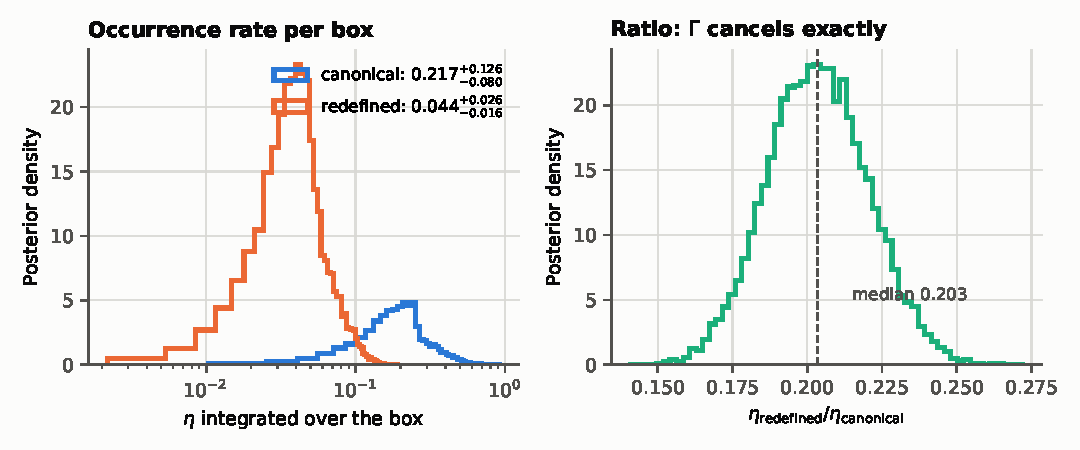
\includegraphics[width=\textwidth]{figOccurrencePosterior.pdf}
\caption{Left: the occurrence rate integrated over each selection box. Right: their ratio, whose
posterior is much tighter because the normalisation $\Gamma$ cancels exactly, leaving only the
shape parameters $\alpha$ and $\beta$.}
\end{figure}

\begin{figure}[htbp]
\centering
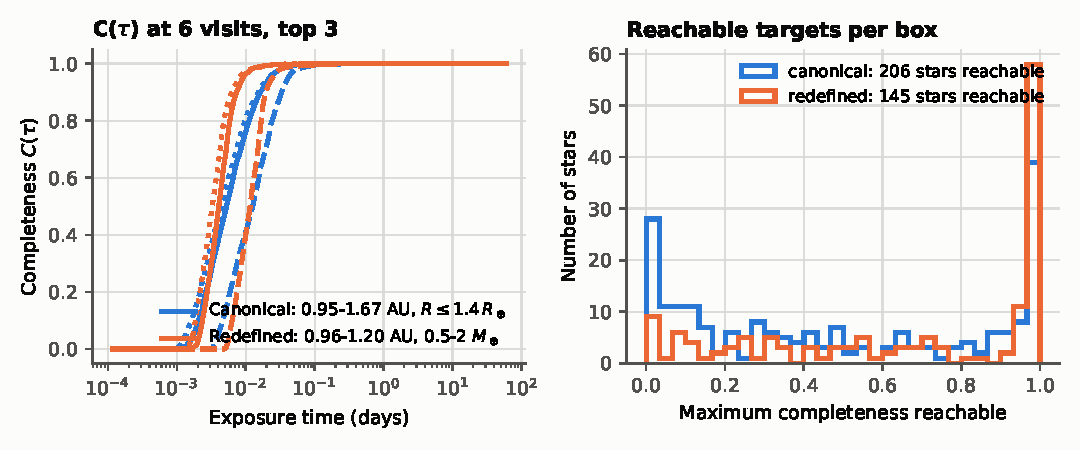
\includegraphics[width=\textwidth]{figCompleteness.pdf}
\caption{Left: completeness against exposure time for the three best targets under both box
definitions. Right: the distribution of reachable completeness. The redefined box gives
\emph{higher} peak completeness (@@COMPREDEFMAX@@ versus @@COMPCANONMAX@@) but reaches far
fewer stars (@@COMPREDEF@@ versus @@COMPCANON@@) --- the two competing effects of truncating the
outer habitable zone.}
\end{figure}

\begin{figure}[htbp]
\centering
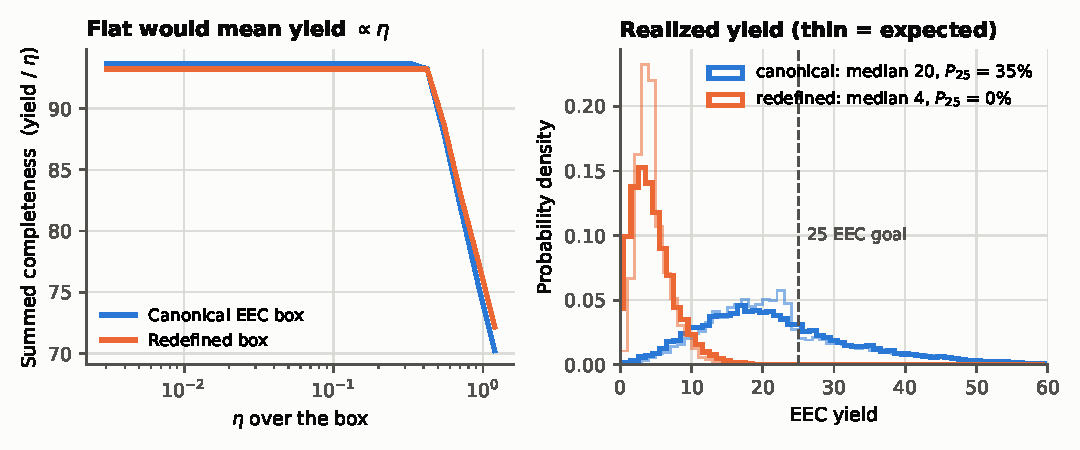
\includegraphics[width=\textwidth]{figYieldPrediction.pdf}
\caption{Left: summed completeness against $\eta$. Were yield proportional to $\eta$ this curve
would be flat; its decline is the characterization burden consuming search time. Right: the
yield distributions marginalised over the occurrence posterior. The heavy curves are the
\emph{realized} yield, a Poisson draw per posterior sample, which is the quantity plotted in
Fig.~10 of Stark et al.\ (2024) and the quantity $P_{25}$ is computed from; the thin curves are
the expected yield $E[N|\eta]$, narrower because they carry the $\eta$ posterior alone without
counting statistics on top.}
\label{fig:yieldprediction}
\end{figure}

\begin{table}[htbp]
\centering
\small
\begin{tabular}{lrr}
\toprule
& \textbf{Canonical box} & \textbf{Redefined box} \\
\midrule
Habitable zone (scaled AU) & 0.95--1.67 & 0.96--1.20 \\
Planet selection & $R \leq 1.4\,R_\oplus$ & $0.5$--$2\,M_\oplus$, $R=M^{0.27}$ \\
Occurrence $\eta$ & $@@ETACMED@@^{+@@ETACUP@@}_{-@@ETACDN@@}$ &
  $@@ETARMED@@^{+@@ETARUP@@}_{-@@ETARDN@@}$ \\
Stars with non-zero completeness & @@COMPCANON@@ & @@COMPREDEF@@ \\
Peak completeness & @@COMPCANONMAX@@ & @@COMPREDEFMAX@@ \\
Median expected yield & @@CANONMED@@ & @@REDEFMED@@ \\
Mean expected yield & @@CANONMEAN@@ & @@REDEFMEAN@@ \\
90\% interval & @@CANONP5@@--@@CANONP95@@ & @@REDEFP5@@--@@REDEFP95@@ \\
$P(\geq 25$ candidates$)$ & @@CANONP25@@\% & @@REDEFP25@@\% \\
\bottomrule
\end{tabular}
\caption{Headline results for the baseline 6\,m LUVOIR-B-like design. The survey uses
@@SURVEYSTARS@@ stars from a screened pool of @@CALSTARS@@.}
\end{table}

\subsection{The central number}

The occurrence ratio between the boxes is
$@@OCCRATIO@@^{+@@OCCRATIOUP@@}_{-@@OCCRATIODN@@}$, and it decomposes: narrowing the habitable
zone contributes a factor of about $0.32$ and the mass selection a further $0.63$. Narrowing the
habitable zone dominates, because it cuts the log-period width to roughly 40\% and because
$\beta > 0$ weights the outer habitable zone more heavily.

The \emph{yield} ratio is $@@YRATIO@@^{+@@YRATIOUP@@}_{-@@YRATIODN@@}$ --- about 38\% larger
than the occurrence ratio. Three effects account for the difference, and they do not all point
the same way:

\begin{enumerate}
\item \textbf{Freed characterization time.} Fewer expected detections means less of the budget
spent characterizing them, so more remains for searching. This raises the ratio.
\item \textbf{The faintest planets are removed.} Truncating at 1.20 scaled AU removes planets
that are a factor $(1.67/1.20)^2 \approx 1.9$ fainter than those at the inner edge and sit
closest to the noise floor. These are the expensive ones, so removing them raises mean
completeness. This raises the ratio.
\item \textbf{Distant targets are lost.} For stars beyond roughly 10--15~pc, only the outer
habitable zone clears the inner working angle at all, so truncation removes those stars from the
survey entirely --- @@COMPREDEF@@ stars remain reachable against @@COMPCANON@@. This lowers the
ratio.
\end{enumerate}

The first two outweigh the third. This is worth stating plainly because the sign is not
obvious in advance, and an occurrence-only rescaling --- which would have given
@@OCCRATIO@@ --- gets it wrong in a direction that cannot be guessed without running the
optimization.

\subsection{What it means for HWO}

Under the redefined selection the baseline 6\,m design delivers a median of @@REDEFMED@@
exoEarth candidates, with a 90\% interval of @@REDEFP5@@--@@REDEFP95@@. The probability of
reaching the Astro2020 benchmark of 25 falls from @@CANONP25@@\% to @@REDEFP25@@\%: not reduced,
but effectively eliminated. If the habitable zone really is as narrow as $0.96$--$1.20$~AU and
the sample of interest really is $0.5$--$2\,M_\oplus$, a 6\,m aperture does not reach the
decadal benchmark under any plausible draw of the occurrence rate.

\section{Limitations}

These are the things a reader should weigh before using these numbers.

\begin{itemize}
\item \textbf{The coronagraph is parametrized, not simulated.} $\Upsilon_c$ and $\zeta$ are
smooth functions of separation fitted to three published anchors, not the two-dimensional maps
AYO interpolates. The calibration factor of @@CALFACTOR@@ bounds the resulting error on the
absolute scale; ratios between boxes, computed within the same implementation, are considerably
more robust than either absolute yield.
\item \textbf{The target catalog is a reconstruction.} It reproduces HPIC's construction and
limits but is not HPIC, and the Hipparcos supplement derives $T_{\rm eff}$ and $L$ from
photometry rather than spectroscopy. Spot checks against $\alpha$~Cen~A agree to a few percent
in luminosity.
\item \textbf{Single-visit completeness.} Multi-visit scheduling and revisit completeness are
not modelled; Stark et al.\ (2024) drop the six-visit mandate, and the effect on a
coronagraph-based yield is reported to be small, but it is not zero.
\item \textbf{The occurrence posterior is prior-dominated in shape.} $\alpha$ and $\beta$ are
constrained by the SAG13 fit, not re-inferred from Kepler DR25. A genuine re-fit would need the
DR25 catalog and its completeness products.
\item \textbf{Exozodi is a fixed 3 zodis} and the local zodiacal surface brightness is the
tabulated average rather than an ecliptic-latitude-dependent model. Stark et al.\ show exozodi
\emph{distribution} uncertainty costs roughly 4\% of the yield.
\item \textbf{Albedo is fixed at $A_G = 0.2$.} The albedo distribution that Stark et al.\ find
costs roughly 15\% of the expected yield is not modelled, which is part of why the
distributions here are narrower than theirs.
\end{itemize}

\section{Reproducing this}

The project is a seven-step vaibify pipeline in \texttt{/workspace/yields}. Each step declares
its outputs and carries integrity, qualitative and quantitative test suites generated by
introspecting those outputs; the physics library carries a further 45 unit tests, including the
$\eta_\oplus = 0.24$ anchor, the Lambert~$W$ coefficient, and the linear/sub-linear $\eta$ pair.
Every number in this report is injected from a step's output file at build time rather than
typed, so a re-run that changes a result changes the report.

\begin{table}[htbp]
\centering
\small
\begin{tabular}{llp{8.4cm}}
\toprule
\textbf{Step} & \textbf{Name} & \textbf{Produces} \\
\midrule
A01 & buildTargetCatalog & Gaia DR3 + Hipparcos target list, @@CATROWS@@ stars \\
A02 & modelCoronagraph & Mission parameters and coronagraph profiles \\
A03 & calibrateToStark & Throughput calibration against the published 22.5 \\
A04 & computeCompleteness & $C(\tau)$ per star, per selection box \\
A05 & optimizeSurvey & Equal-slope allocation and baseline yield \\
A06 & sampleOccurrencePosterior & \texttt{emcee} posterior over the rate law \\
A07 & predictRedefinedYield & Marginalised yield distributions and the ratio \\
\bottomrule
\end{tabular}
\caption{Pipeline steps. Cross-step inputs are declared as tokens in the project file so the
dependency graph is explicit.}
\end{table}

\section*{References}
\small
\begin{itemize}
\item Stark, C.~C., et al.\ 2014, ApJ 795, 122 --- AYO and the equal-slope method.
\item Stark, C.~C., et al.\ 2019, JATIS 5, 024009 (arXiv:1904.11988) --- exposure-time
equations, coronagraph performance, the exoEarth yield landscape.
\item Stark, C.~C., et al.\ 2024, JATIS 10, 034006 (arXiv:2405.19418) --- the HWO baseline
mission, Tables 1 and 2, and the yield uncertainty budget.
\item Bryson, S., et al.\ 2021, AJ 161, 36 --- Kepler DR25 occurrence rates.
\item Kopparapu, R.~K., et al.\ 2013, ApJ 765, 131 --- habitable zone boundaries.
\item Chen, J., \& Kipping, D. 2017, ApJ 834, 17 --- mass--radius relation.
\item Torres, G. 2010, AJ 140, 1158 --- bolometric corrections.
\item Ballesteros, F.~J. 2012, EPL 97, 34008 --- $B\!-\!V$ to $T_{\rm eff}$.
\item Gaia Collaboration 2023, A\&A 674, A1 --- Gaia DR3.
\end{itemize}

\end{document}
